\section{Aufgabenstellung}
Unsere Aufgabenstellung ist es einen Workflow zur Urlaubsgenehmigung in einem Unternehmen nachzubilden. Dabei sollen bestimmte Geschäftsregeln (s. Abschnitt \ref{Geschäftsregeln}) auf eine beispielhafte Personalhierarchie (s. Abschnitt \ref{Personalhierarchie}) abgebildet werden.

Ziel unserer Aufgabe ist die Entwicklung einer prototypischen Anwendung, die den Urlaubsgenehmigungsprozess in einem BPMN-Diagramm zeigt und eine Interaktion mit dem Endanwender ermöglicht.

\subsection{Geschäftsregeln}
\label{Geschäftsregeln}

Für den Urlaubsgenehmigungsprozess in unserem Beispielunternehmen gelten die folgenden Regeln:\footnote{Die Regeln wurden aus der Aufgabenstellung "`Aufgabe Urlaubsgenehmigung jBPM.pdf"' übernommen}
\begin{enumerate}
	\item Reicht ein Mitarbeiter einen Urlaubsantrag ein, so ist dieser bei 20 Werktagen oder weniger
	immer an den direkten Vorgesetzten weiter zu leiten und durch diesen zu genehmigen oder
	abzulehnen. Hat der direkte Vorgesetzte nach drei Tagen noch nicht über den Urlaubsantrag
	entschieden (z.B. weil er nicht da ist), wird der Urlaubsantrag eine Ebene höher geleitet.
	\item Wird ein Urlaub von mehr als 20 Werktagen beantragt, so muss dieser zusätzlich vom Leiter der
	Personalabteilung genehmigt werden.
	\item Wenn ein Urlaubsantrag abgelehnt wurde, ist der Mitarbeiter in Kenntnis zu setzen.
	\item Wenn ein Urlaubsantrag genehmigt wurde, ist er sofort an zuständigen Sachbearbeiter in der
	Personalabteilung weiter zu leiten. Diese prüft, ob noch genügend Urlaubstage zur Verfügung
	stehen. Ist dies nicht der Fall und es handelt sich nicht um Sonderurlaub (siehe unten), wird der
	Urlaubsantrag an den Vorgesetzen zurückgegeben und kann nicht genehmigt werden.
	\item Sonderurlaub kann gewährt werden bei Umzug (max. 1 Tag), Geburt- oder Todesfall (max. 2
	Tage) oder als Bonus (max. 3 Tage). Sonderurlaub wird nicht auf die normalen Urlaubstage
	angerechnet.
	\item Sonderurlaubsanträge für Umzug und Geburts- oder Todesfälle sind immer automatisch zu
	genehmigen. Ein Bonus-Urlaub ist durch Vorgesetzten und den Leiter der Personalabteilung zu
	genehmigen.
	\item Über den Urlaub eines Vorstandsmitglieds entscheidet der Vorstandsvorsitzende. Urlaubsanträge
	des Vorstandsvorsitzenden werden dem stellvertretenden Vorstandsvorsitzenden vorgelegt.
	Urlaube von Vorstandsmitgliedern von weniger als 5 Tagen müssen nicht genehmigt (aber
	natürlich in der Personalabteilung vermerkt werden. Bei Vorstandsmitgliedern wird ein
	Überziehen des zur Verfügung stehenden Urlaubs um maximal 3 Tage geduldet.
	\item Normale Mitarbeiter erhalten 30 Tage Urlaub pro Jahr, Mitglieder des Vorstands 25 Tage.
\end{enumerate}

\subsection{Personalhierarchie}
\label{Personalhierarchie}

Im Beispielunternehmen ist die folgende Personalhierarchie gegeben:
\begin{figure}[H]
\centering
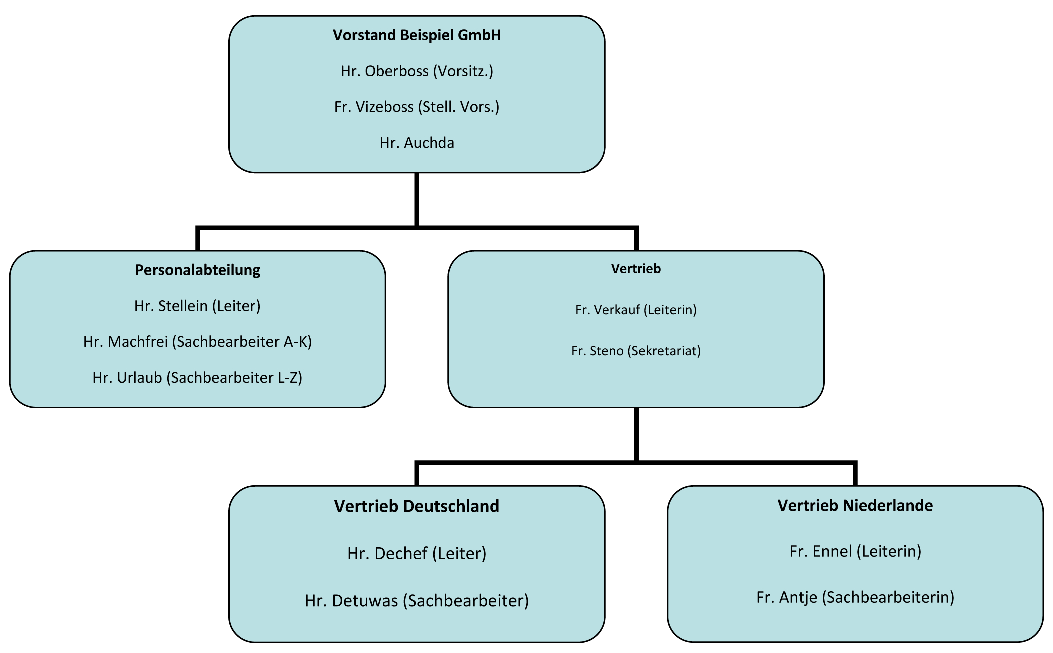
\includegraphics[width=1.0\linewidth]{Bilder/Hierarchie}
\caption[]{Personalhierarchie unseres Beispielunternehmens\footnotemark}
\label{fig:Hierarchie}
\end{figure}
\footnotetext{Quelle: Aufgabe Urlaubsgenehmigung jBPM.pdf}

In der Personalhierarchie gibt es einige erwähnenswerte Besonderheiten. In der Personalabteilung gibt es zwei Sachbearbeiter mit unterschiedlichen Zuständigkeiten. Herr Machfrei ist für die Mitarbeiter, deren Nachname mit einem Buchstaben zwischen A und K beginnen, zuständig. Herr Urlaub bearbeitet die Übrigen, deren Nachnamen mit L bis Z beginnen.\\
Des Weiteren ist der Vorgesetzte im abteilungsübergreifenden Falle immer Leiter der entsprechend höheren Abteilung. Gleiches gilt für den stellvertretenden Vorgesetzten. Für die Vorstandsebene ergibt sich die Besonderheit, dass der "`Vorgesetzte"' des Oberbosses der Vizeboss ist.
Der stellvertretende Vorgesetzte des Oberbosses ist somit wiederum der Oberboss selbst. Gleiches gilt für den Vizeboss, dessen stellvertretender Vorgesetzter er selbst ist.


